\section{Experimentelles Vorgehen}
In der Versuchsdurchführung soll in jeweils drei Versuchsdurchläufen der Gefrierpunkt von destilliertem Wasser sowie von einer Salzlösung (in diesem Fall: $NaNO_3$) festzustellen. Zusätzlich soll der Temperaturverlauf des Wassers/der Lösung alle 5 Sekunden protokolliert werden. Die Temperatur soll mithilfe eines Termistors bestimmt werden, der im Anschluss kalibriert wird. 

\begin{center}
\begin{figure}
\centering
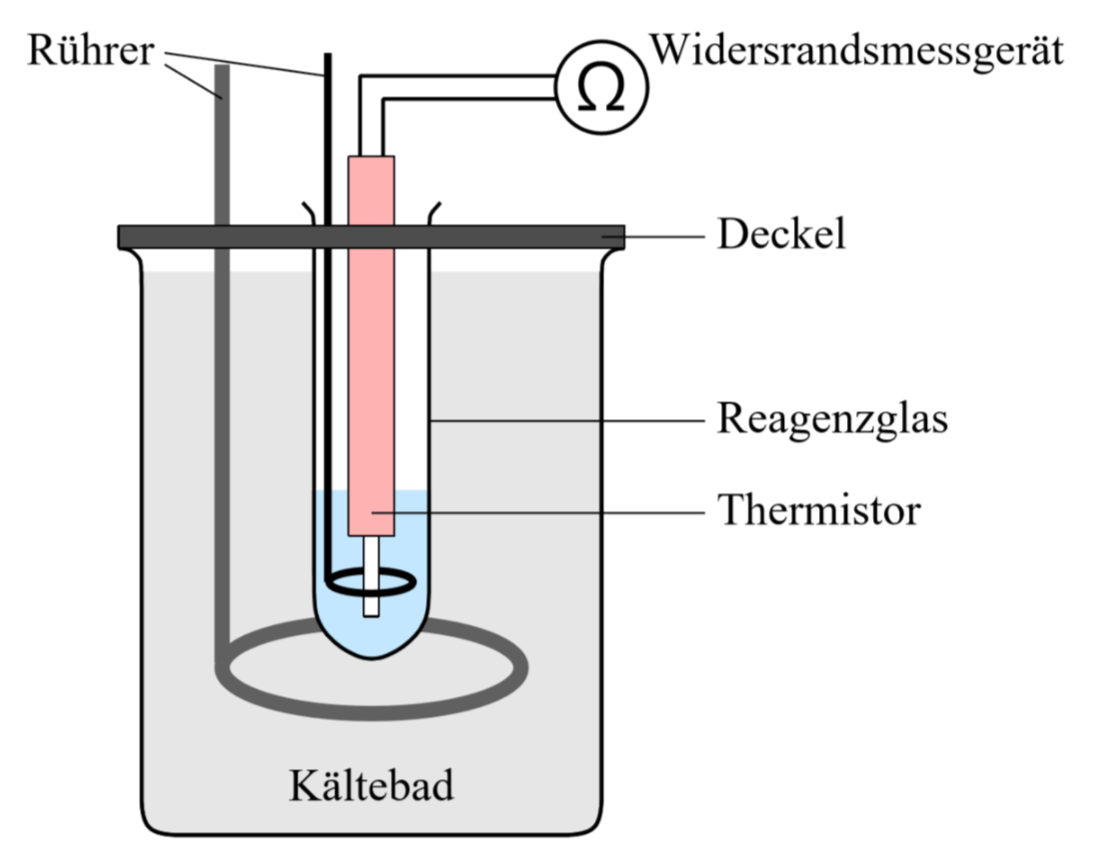
\includegraphics[scale=0.8]{Bilder/Versuchsaufbau.png}
\caption{Versuchsaufbau}
\label{fig:aufbau}
\end{figure}
\end{center}